\documentclass[11pt, french]{article}
\usepackage{calc}
\usepackage{eso-pic}

\newlength{\PageFrameTopMargin}
\newlength{\PageFrameBottomMargin}
\newlength{\PageFrameLeftMargin}
\newlength{\PageFrameRightMargin}

\setlength{\PageFrameTopMargin}{1.5cm}
\setlength{\PageFrameBottomMargin}{1cm}
\setlength{\PageFrameLeftMargin}{1cm}
\setlength{\PageFrameRightMargin}{1cm}

\makeatletter

\newlength{\Page@FrameHeight}
\newlength{\Page@FrameWidth}

\AddToShipoutPicture{
  \thinlines
  \setlength{\Page@FrameHeight}{\paperheight-\PageFrameTopMargin-\PageFrameBottomMargin}
  \setlength{\Page@FrameWidth}{\paperwidth-\PageFrameLeftMargin-\PageFrameRightMargin}
  \put(\strip@pt\PageFrameLeftMargin,\strip@pt\PageFrameTopMargin){
    \framebox(\strip@pt\Page@FrameWidth, \strip@pt\Page@FrameHeight){}}}

\makeatother
%%%%%%%%%%%%%%%%%%%%%%%%%%%%%%%%%%%%%%%%%%%%%%%%%%%%%
% Importation des paquets
%%%%%%%%%%%%%%%%%%%%%%%%%%%%%%%%%%%%%%%%%%%%%%%%%%%%%
\usepackage[utf8]{inputenc}
\usepackage{helvet}
\usepackage{natbib}
\usepackage{graphicx}
\usepackage{libertine}
\usepackage{eso-pic}
\usepackage{hyperref} % allow to write hyperlink (open the url)
\usepackage{titlesec} % allow to change fontsize of the different section
\usepackage{tabularx} % allow to create tables with fixed length
\usepackage{listings} % code highlighting
\usepackage{xcolor}
\usepackage{amsmath}
\usepackage{amssymb}
\usepackage{multirow}

\usepackage[a4paper,margin=1in]{geometry}
\definecolor{LightGray}{gray}{0.9}


%%%%%%%%%%%%%%%%%%%%%%%%%%%%%%%%%%%%%%%%%%%%%%%%%%%%%
% Definition des commandes
%%%%%%%%%%%%%%%%%%%%%%%%%%%%%%%%%%%%%%%%%%%%%%%%%%%%%
% Permet de définir une image en arrière plan
\newcommand\BackgroundPic{%
\put(0,0){%
\parbox[b][\paperheight]{\paperwidth}{%
\vfill
\centering
\includegraphics[width=\paperwidth,height=\paperheight]{background-42-ai.png}%
\vfill
}}}

% Définition de la commande pour faire un snippet de code inline
\newcommand{\inlsnippet}[1]{\colorbox{gray!10}{\mbox{\textcolor{pink}{#1}}}}

% Modification of the style of hyperlink, to be visible
\hypersetup{
    colorlinks=true,
    linkcolor=blue,
    filecolor=magenta,      
    urlcolor=cyan,
}

%%%%%%%%%%%%%%%%%%%%%%%%%%%%%%%%%%%%%%%%%%%%%%%%%%%%%%%%%%%%%%%%%%%%%%%%%%%
% Definition of black backgrounded Python code snippet
%%%%%%%%%%%%%%%%%%%%%%%%%%%%%%%%%%%%%%%%%%%%%%%%%%%%%%%%%%%%%%%%%%%%%%%%%%%
\definecolor{pink}{HTML}{ff33cc}
\definecolor{codewhite}{HTML}{ffffff}
\definecolor{codegreen}{HTML}{00e600}
\definecolor{codelemon}{HTML}{99ff99}
\definecolor{codegray}{HTML}{bfbfbf}
\definecolor{codepurple}{HTML}{9933ff}
\definecolor{codeblue}{HTML}{0099ff}
\definecolor{codered}{HTML}{ff3333}
\definecolor{bg}{HTML}{000000}

\lstdefinestyle{nightly}{
    language=Python,
    backgroundcolor=\color{bg},   
    commentstyle=\fontfamily{cmss}\color{codegreen},
    keywordstyle=\fontfamily{cmss}\color{codeblue},
    otherkeywordstyle=\fontfamily{cmss}\color{codered},            
    numberstyle=\fontfamily{cmss}\small\color{codegray},
    stringstyle=\fontfamily{cmss}\color{codepurple},
    basicstyle=\fontfamily{cmss}\small\color{codewhite},
    emph={def,is,not,in,False,True,as,and,or,from},
    emphstyle={\fontfamily{cmss}\small\color{pink}},
    emph={[2]MyClass,__init__,__repr__,__print__},
    emphstyle={[2]\fontfamily{cmss}\small\color{codered}},
    emph={[3]str,float,tuple,int,list},
    emphstyle={[3]\fontfamily{cmss}\small\color{codelemon}},
    breakatwhitespace=false,         
    breaklines=true,                 
    captionpos=b,                    
    keepspaces=true,                 
    numbers=left,                    
    numbersep=5pt,                  
    showspaces=false,                
    showstringspaces=false,
    showtabs=false,                  
    tabsize=2
}
%%%%%%%%%%%%%%%%%%%%%%%%%%%%%%%  End of definition  %%%%%%%%%%%%%%%%%%%%


%%%%%%%%%%%%%%%%%%%%%%%%%%%%%%%%%%%%%%%%%%%%%%%%%%%%%
% Titre, date, auteur
%%%%%%%%%%%%%%%%%%%%%%%%%%%%%%%%%%%%%%%%%%%%%%%%%%%%%

\author{} %\author{42-AI}
\title{Practise sheet}
%\maketitle

%%%%%%%%%%%%%%%%%%%%%%%%%%%%%%%%%%%%%%%%%%%%%%%%%%%%%
% Début du document
%%%%%%%%%%%%%%%%%%%%%%%%%%%%%%%%%%%%%%%%%%%%%%%%%%%%%
\begin{document}


%%% >>>>> Page de garde
\vspace*{2cm}
\begin{center}
    \textsc{\fontsize{40}{48} \bfseries Practise Sheet 4}\\[0.6cm]
    \textsc{\fontsize{40}{48} \bfseries Analysis}\\[0.3cm]
\end{center}
\vspace{3cm}

\begin{figure}[!h]
\center

\includegraphics[scale=0.5]{logo-42-ai.png}
\label{fig:1st_page_logo_42ai}
\end{figure}

\vspace*{2cm}
\begin{center}
    \textsc{\fontsize{32}{48} \bfseries Fonctions polynomiales du second degré}\\[0.6cm]
\end{center}
\vspace{3cm}

\pagenumbering{gobble}
\newpage


%%% >>>>> Document body

\section*{Objectifs:}
L'objectif principal de cette série d'exercices est de vous entraîner à manipuler des fonctions polynomiales de degré 2 et supérieure.
Vous rencontrerez les polynômes dans un premier temps pour la création de modèles polynomiaux, un peu dans les méthodes de régularisation (Ridge regularization, Lasso regularization ou encore ElasticNet) ou encore pour certaine notion en Reinforcement Learning.



\section*{Exercice 1:}
Dans cette exercice vous vous entraînerez à déduire des informations sur des polynômes simples en observant les représentations graphiques.\\
L'objectif est que vous compreniez l'influence des différents coefficients au sein des polynômes.


Dans le cas des fonctions affines l'influence des coefficients est plus facilement distinguable:
\begin{itemize}
    \item une valeur positive de l'ordonnée à l'origine (ce que l'on note $b$ usuellement dans l'équation $f(x) = ax+b$) entraîne une translation positive, alors qu'une valeur négative de $b$ conduit à une translation vers les négatifs.
    \item une augmentation du coefficient directeur quant à lui conduit à une pente "plus raide" de la droite, alors qu'une valeur positive et qui tend vers $0$, "adoucit" la pente. Une valeur négative du coefficient directeur fait que la pente "devient une descente".
\end{itemize}

\begin{figure}[!h]
\center
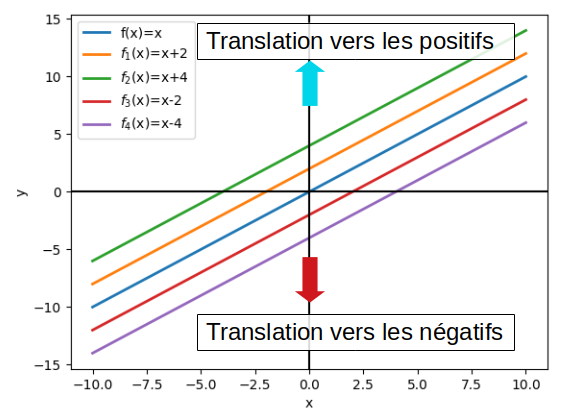
\includegraphics[scale=0.49]{assets/serie_4_exo_1_figure_1.png}
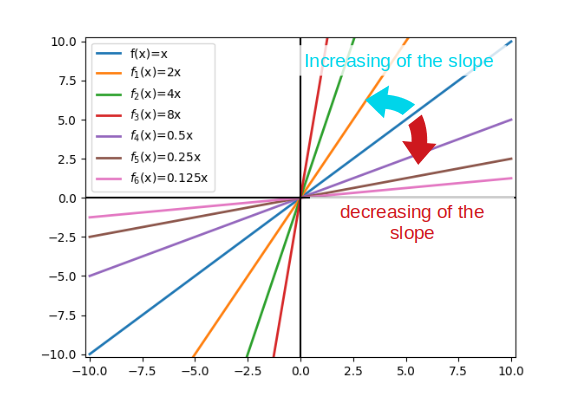
\includegraphics[scale=0.54]{assets/serie_4_exo_1_figure_2.png}
\label{fig:p_s_4_exo1-fig1+2}
\end{figure}

L'analyse que l'on vient de faire est vraiment faite "avec les mains" mais elle décrit le type d'intuition que l'on va travailler dans cette exercice.

\subsection*{Questions:}
Vous devez associer les différentes courbes aux expressions données dans les 2 figures suivantes.

\subsection*{Remarques:}
Réfléchissez à l'influence qu'à le coefficient $a$ dans l'expression:
\begin{equation*}
    f(x) = ax^2
\end{equation*}
Et également, réfléchissez à l'impacte de $c$ dans l'expression:
\begin{equation*}
    f(x) = x^2+c
\end{equation*}

\begin{figure}[!h]
\center
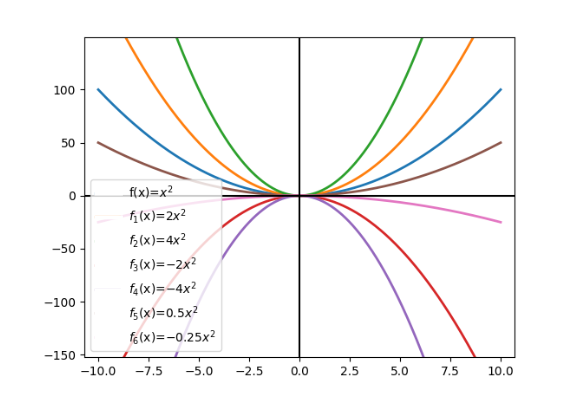
\includegraphics[scale=1]{assets/serie_4_exo_1_figure_3.png}
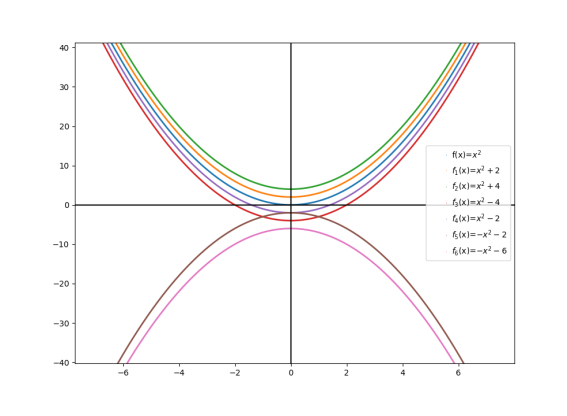
\includegraphics[scale=1]{assets/serie_4_exo_1_figure_4.png}
\label{fig:p_s_4_exo1-fig1+2}
\end{figure}

\textit{Évidemment vous pouvez vous aider en représentant à l'aide de \inlsnippet{matplotlib.pyplot}  différentes courbes de fonctions du type $ax^2$ et $x^2+c$.}


\section*{Exercice 2}

\subsection*{Partie 1:}
Dans cette exercice nous allons nous intéresser à la résolution des équations du type:
\begin{equation*}
    ax^2+bx+c = 0
\end{equation*}

Cette équation se traduit graphiquement par l'intersection de la fonction $ax^2+bx+c$ avec l'axe des abscisses.\\
Les valeurs de x pour lesquelles le polynôme s'annule sont appelées les racines du polynôme.\\
Noter également l'équivalence entre le fait de déterminer les racines d'un polynôme $P(x)$ et résoudre l'équation $P(x) = 0$.

\subsubsection*{Rappel:}
Il vous faut d'abord calculer le discriminant et en fonction du signe de celui-ci vous pouvez dire s'il existe 2, une ou aucunes racines réelles. Puis, si la(/les) racine(/s) existe(nt), une formule permet de la/les calculer.

\begin{enumerate}
    \item Déterminer les racines des polynômes suivants lorsqu'elles existent.
\end{enumerate}

\begin{equation*}
    \begin{matrix}
    P_1(x) = x^2 + 4x + 1 & P_2(x) = 2x^2 - x +6 & P_3(x) = -2x^2 - 4x - 7 \\
    P_4(x) = -x^2 + 2x + 3 & P_5(x) = \frac{1}{3}x^2 + 2x - 3 & P_6(x) = 2x^2 + 7x + 11 \\
    P_7(x) = -2x^2 + 3x - 4 & P_8(x) = \frac{1}{2}x^2 - 4x + 8 & P_9(x) = -x^2 - 2x +35
    \end{matrix}
\end{equation*}

\begin{enumerate}
    \setcounter{enumi}{1}
    \item Représenter les différents polynômes et vérifier graphiquement l'existence et les valeurs des racines des polynômes en ayant.
\end{enumerate}

\subsection*{Partie 2:}
\begin{enumerate}
    \item Réaliser une fonction python permettant de calculer le discriminant et une seconde fonction permettant de calculer les possibles racines d'un polynôme.
\end{enumerate}
\begin{lstlisting}[style=nightly]
    def discriminant(poly):
        """
        Parameter:
            poly : expression of a polynom (ax**2 + b*x + c).
        Description:
            Function calculates the discriminant.
        Return:
            the value of the discriminant.
        """
            'Your code, you may need to use sympy.coef(x**2) or sympy.coef(x)'
    
    def polynom_root(poly):
        """
        Parameter:
            poly : expression of a polynom (ax**2 + b*x + c).
        Description:
            Function calculates the discriminant.
        Return:
            the value of the discriminant.
        """
            'Your code, but do not use a solver (sympy.solve, solvset)' 
    
    import sympy as sy
    x = sy.Symbol('x')
    P1 = -3*x**2 + 2*x + 1
    discriminant(P1)
    # Output:
    16
    polynom_root(P1)
    # Output:
    [-1/3, 1]
\end{lstlisting}

\begin{enumerate}
    \setcounter{enumi}{1}
    \item Calculer les racines, si elles existent, des polynômes suivant. Tracer leurs représentations graphiques et vérifier l'existence et les valeurs des racines.
\end{enumerate}
\begin{equation*}
    \begin{matrix}
    P_{10}(x) = 2x^2 - 8x -10  & P_{11}(x) = 2x^2 -14x + 12 & P_{12}(x) = -\frac{1}{2}x^2 + 5x -12.5  \\
    P_{13}(x) = 4x^2 + 4x - 8 & P_{14}(x) = 3x^2 - 2x +2.4  & P_{15}(x) = 4(x-1)^2-16
    \end{matrix}
\end{equation*}
\vspace{1cm}

\section*{Exercice 2}

\subsection*{Partie 1:}
Il n'y a pas de motivation directe (à la connaissance de l'auteur) à savoir construire le tableau de signes et de variations d'une fonction pour le machine learning. Ce que vous allez apprendre ici, en plus de renforcer votre manipulation des polynômes du second degré qui est important pour vous, est un outil mathématique classique, étudié au lycée.

\noindent\rule{\textwidth}{1pt}
\subsubsection*{Exemple: Tableau de signes}
Afin de construire un tableau de signes d'une fonction $f$, il faut résoudre 3 équations:
\begin{align*}
    f(x) < 0 \\
    f(x) > 0 \\
    f(x) = 0
\end{align*}
L'équation sur laquelle on peut sauter dessus est $f(x) = 0$.\\
Prenons comme fonction $f$:
\begin{equation*}
    f(x) & = & 2x^2-4x-16
\end{equation*}
Résolvons $f(x) = 0$:
\begin{equation*}
    \Delta & = & (-4)^2 -4\times 2 \times (-16)\\
    & = & 16 + 128\\
    & = & 144
\end{equation*}
Le discriminant est positif, il y a donc 2 racines réelles:
\begin{equation*}
    \begin{matrix}
        x_{1} & = & \frac{-4 -\sqrt{144}}{4} & x_{2} & = & \frac{-4 +\sqrt{144}}{4} \\
              & = & -2            &       & = & 4 
    \end{matrix}
\end{equation*}
Ainsi, $f(x) = 0$ pour $x = \{-2; 4\}$.\\
Il reste alors à déterminer les solutions des équations:
\begin{align*}
    f(x) < 0 \\
    f(x) > 0
\end{align*}
À partir d'ici, 2 manières de faire son possible. La première se base sur la connaissance des variations d'un polynôme du second degré à partir du signe du coefficient du terme $x^2$ et du signe de $\Delta$ (voir fiche).
La seconde consiste à passer par la forme factorisée du polynôme. La forme factorisée s'exprime à partir des racines du polynôme:

\begin{equation*}
    f(x) = (x-x_1)(x-x_2)
\end{equation*}

Ainsi:

\begin{align*}
f(x) > 0 \text{ si } \Big\{
\begin{matrix}
(x+2) > 0 \text{\hspace{0.5cm} et \hspace{0.5cm}} (x - 4) > 0 \\
(x+2) < 0 \text{\hspace{0.5cm} et \hspace{0.5cm}} (x - 4) < 0
\end{matrix} \\
f(x) < 0 \text{ si } \Big\{
\begin{matrix}
(x+2) < 0 \text{\hspace{0.5cm} et \hspace{0.5cm}} (x - 4) > 0 \\
(x+2) > 0 \text{\hspace{0.5cm} et \hspace{0.5cm}} (x - 4) < 0
\end{matrix}
\end{align*}

Il faut alors résoudre les systèmes d'équations pour obtenir les intervalles où $f$ est positive et où $f$ est négative.

Dans notre cas, f est positive pour $x\in ]-\infty;-2[\cup]4;+\infty[$ et $f$ est négative pour $x\in ]-2;4[$.

D'où le tableau de signes:
\begin{table}[!h]
    \centering
    \begin{tabular}{|c | c c c c c|}
        \hline
        x             &  $-\infty$ & $-2$ &   & $4$ & $+\infty$ \\\hline
        signe de f(x) &    +       &        $|$     & - &       $|$     &   +      \\\hline     
    \end{tabular}
\end{table}

Il est également très courant de voir le tableau de variations de la fonction accompagner le tableau de signe. 

\noindent\rule{\textwidth}{1pt}

\subsubsection*{Questions:}
\begin{itemize}
    \item Dresser (feuille + crayon) le tableau de signes des polynômes:
\end{itemize}
\begin{equation*}
    \begin{matrix}
    g(x) = 9x^2+24x+16 & & h(x) = 2x^2-5x+6
    \end{matrix}
\end{equation*}

\begin{itemize}
    \item Vérifier vos résultats en utilisant la méthode \inlsnippet{sympy.solevet} 
(\href{https://docs.sympy.org/latest/modules/solvers/solveset.html}{page vers solveset}).
\end{itemize}

\subsubsection*{Pour aller plus loin:}
\begin{itemize}
\item Vous pouvez vous amuser à coder une fonction qui donne le tableau de signes du polynôme du second degré donné en paramètre de celle-ci.
\item De même pour le tableau de variations, vous aurez besoin de déterminer le signe de la dérivée du polynôme.
\end{itemize}

\subsection*{Partie 2:}
La forme factorisée d'un polynôme (si elle existe) permet principalement d'avoir accès directement aux racines (si elles existent) du polynôme.\\
(\textit{Donc un intérêt limité pour le machine learning, mais un B-A-BA pour les polynômes du second degré.})

\begin{itemize}
\item Déterminer, si elle existe, la forme factorisée des polynômes suivants:
\end{itemize}
\begin{align*}
    f(x) = -2x^2+3x-4 \\
    g(x) \frac{1}{2}x^2 -4x +8 \\
    h(x) = -x^2 -2x +35
\end{align*}
\begin{itemize}
    \item Vérifier vos résultats en utilisant la méthode \inlsnippet{sympy.factor} 
(\href{https://docs.sympy.org/latest/tutorial/simplification.html}{page vers factor}).
\end{itemize}
\vspace{1cm}


\section*{Exercice 3:}
à venir...
\subsection*{Partie 1:}

\subsection*{Partie 2:}

%\begin{lstlisting}[style=nightly]
%import numpy as np
%def test_function:
 %   """
 %   Description..
 %   """
 %   for i in range(0,5):
 %       list()
 %       int()
 %       return
 %   
 %   # comment
 %   x = 2
 %   test_function()
%\end{lstlisting}

\end{document}
%%%%%%%%%%%%%%%%%%%%%%%%%%%%%%%%%%%%%%%%%%%%%%%%%%%%%